\section{Einführung}
In diesem Versuch wird die Wirkungsweise des Geiger-Müller-Zählrohrs untersucht.
Dieses ist ein Messinstrument um die Intensität ionisierender Strahlung zu messen.

\section{Theorie}

Bei dem Geiger-Müller-Zählrohr werden elekrtische Impulse erzeugt, wenn $\alpha$-,
$\beta$- oder $\gamma$-Teilchen absorbiert werden.

\begin{figure}[H]
  \centering
  \includegraphics[width=\textwidth]{content/Zählrohr.png}
  \caption{Schematische Darstellung eines Zählrohrs \cite{1}.}
  \label{abb:1}
\end{figure}

Das Zählrohr besteht aus einem Hohlzylinder, der als Kathode fingiert, und in der
Mitte des Zylinders befindet sich ein Draht der die Anode ist. Damit ergibt sich
ein elekrtisches Feld im inneren des Zählrohrs, das mit folgender Formel beschrieben
werden kann.

\begin{equation}
  E(r) = \frac{U}{r \ln{\frac{r_k}{r_a}}}
  \label{eq:1}
\end{equation}

Dabei ist r der Abstand von dem Draht. Außerdem ist das Zählrohr mit einem Gasgemisch
gefüllt, welches aus Argon und Ethylalkohol bestehen kann. Es werden aber auch andere
Gase verwendet. Die Stelle, wo die Strahlung in das Zählrohr eintreten soll muss sehr
dünn sein, damit selbst $\alpha$-Teilchen es durchdringen können. Durch eine Mylar-
Folie ist es wird dies erreicht, da jede Art von Strahlung die durchdringen kann.

Wenn ein Teilchen in das Zählrohr eindringt, bewegt es sich so lange im Gasraum bis
es seine gesamte Energie in Form von Ionisation abgegeben hat. Dieser Vorgang wird als
Primärionisation bezeichnet. Was nach dieser Primärionisation geschiet hängt von der
angelegten Spannung ab.

\begin{figure}[H]
  \centering
  \includegraphics[width=\textwidth]{content/Primärionisation.png}
  \caption{Graphik der in einem Zählrohr erzeugten Elektron-Ionen-Paare als Funktion
  der Spannung \cite{1}.}
  \label{abb:2}
\end{figure}

Bei geringer Spannung, also im 1. Bereich, gehen die meisten erzeugten Elektronen
durch Rekombination verloren bevor sie den Draht erreichen können.

Im 2. Bereich, wenn die Spannung etwas erhöht wird, erreichen fast alle Elektronen
den Anodendraht und der Ionisationsstrom ist proportional zur Energie und Intensität
der Strahlung. Da dieser Ionisationsstrom nur sehr gering ist sind solche Spannungen
nur bei hohen Strahlenintensitäten sinnvoll.

In dem Bereich 3 ist die Spannung bereits so groß, dass die erzeugten Elektronen
so viel Energie aufnehmen können, dass sie selber ionisieren können durch Stoßionisation.
Die dadurch erzeugten Elektronen können auch wieder ionisieren, wodurch die Zahl der Elektronen
lawinenartig zunimmt. Diese \enquote{Lawinen} nennt man Townsend-Lawine. Dieser Vorgang
kann als Ladungsimpuls erfasst werden, welcher noch proportional zu der von dem
einfallenden Teilchen abgegebenen Energie ist. Deshalb können Intensitäts und Energiemessungen
durchgeführt werden.

Nach diesem Proportionalitätsbereich liegt der Bereich in dem das Geiger-Müller-
Zählrohr arbeitet. In der Abbildung \ref{abb:2} ist das der 4. Bereich. Dort sind
die Ladungsimpulse unabhängig zur Primärionisation, da während den Elekronenlawinen
auch Photonen entstehen, die selber wieder Elektronenlawinen im gesamten Zählrohrvolumen
auslösen können. Deshalb sind Energiemessungen nicht mehr möglich, allerdings
kann die freigesetzte Ladung jetzt leicht nachgewiesen werden.\\\\


Die entstandenen Ionen brauchen, aufgrund ihrer größeren Masse, länger um aus dem
Zählrohrvolumen abzuwandern. Deshalb bildet sich vorübergehend eine Positive Raumladung
die dafür sorgt, dass keine Stoßionisation mehr stattfinden kann. In dieser Zeit kann
das Zählrohr kein Teilchen mehr regestrieren. Diese Zeit heißt Totzeit.

Erst wenn alle Ionen neutralisiert wurden und wieder die ursprüngliche Feldstärke wieder
herrscht haben die Ladungsimpulse wieder ihre ursprüngliche Höhe. Davor sind Stoßionisationen
zwar möglich, aber die Ladungsimpulse sind geringer. In Abbildung \ref{abb:3} sind diese
Vorgänge auch graphisch Dargestellt.

\begin{figure}[H]
  \centering
  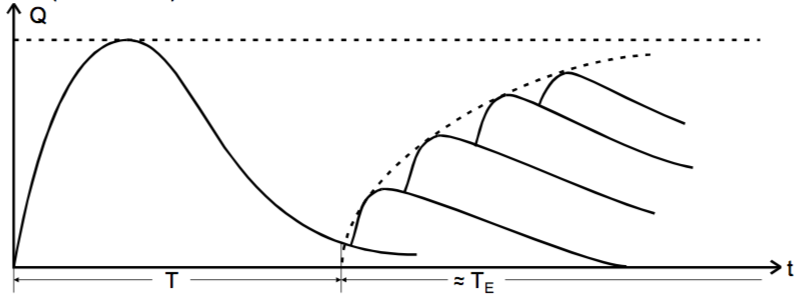
\includegraphics[width=\textwidth]{content/Totzeit.png}
  \caption{Graphische Darstellung der Tot- und Erhohlzeit in Form eines Ladungs-Zeit-Diagramms
  \cite{1}.}
  \label{abb:3}
\end{figure}

Ein Nachteil des Zählrohrs ist, dass es zu Nachentladungen kommen kann. Das bedeutet,
dass die Ionen, beim auftreffen auf den Kathodenmantel, Elektronen freisetzen können.
Diese Elektronen können wieder Elektronenlawinen und somit Ladungsimpulse Auslösen.
Durch den Zusatz von Ethylalkohol wird dieser Effekt gut unterdrückt, denn die
Edelgasionen stoßen mit den Alkoholmolekülen zusammen und dabei werden die Alkoholmoleküle
ionisiert. Also werden die Alkoholionen anstelle der Edelgasionen an der Kathode neutralisiert.
Diese setzen keine Elektronen frei, da die freigesetzte Energie zur Anregung von Schwingungen
der Alkoholmoleküle verbraucht wird.

\begin{figure}[H]
  \centering
  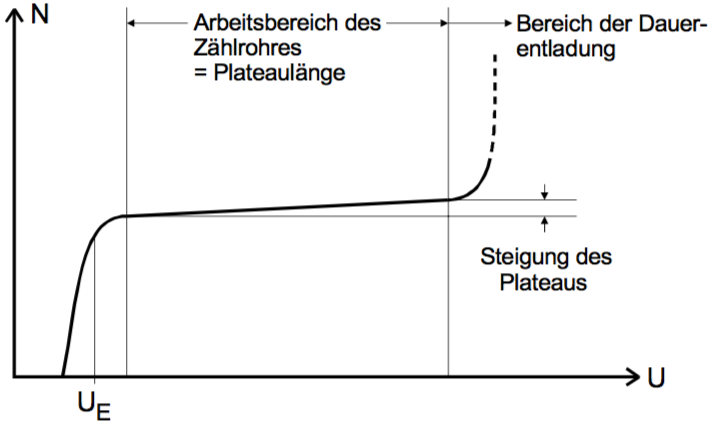
\includegraphics[width=\textwidth]{content/Plateau.png}
  \caption{Darstellung der regestrierten Teilchenzahl bei konstanter Strahlungsintensität
  \cite{1}.}
  \label{abb:4}
\end{figure}

In Abbildung \ref{abb:4} wird deutlich, dass sich bei konstanter Strahlungsintensität
eine Charakteristik ergibt. Der lineare Teil der Kurve heißt Plateau und das ist der
Arbeitsbereich des Zählrohrs. Das Plateau hat eine Steigung, welche sich durch die wenigen
Nachentladungen ergibt, die nicht unterdrückt werden können.

Nach dem Plateau ist die Spannung so hoch, dass die Nachentladungen stark zunehmen
und es kann durch ein einzelnes ionisierendes Teilchen zu einer Dauerentladung kommen.
\\\\

Geladene Teilchen, wie $\alpha$- und $\beta$-Teilchen, können durch ein Zählrohr
gut nachgewiesen werden. Bei Photonen kommt es für das Ansprechverhalten auf die
Energie an, da ihre Wechselwirkung mit Materie sehr gering ist. Hochenergetische
$\gamma$-Quanten können nur bei hoher Intensität gut nachgewiesen werden. Röntgen-Quanten
können vergleichsweise besser mit einem Zählrohr erfasst werden. Bei dem Ansprechverhalten
kommt es auch auf das verwendete Füllgas an.
